%%%%%%%%%%%%%%%%%%%%%%%%%%%%%%%%%%%%%%%%%%%
%%%%%%%%%%%%%%%%%%%%%%%%%%%%%%%%%%%%%%%%%%%
%%%%%%%%%%%%%%% CHAPTER 01 %%%%%%%%%%%%%%%%


\section{Introdução à Automação}

\frame{
\frametitle{Histórico da automação}
\begin{block}{Revolução Industrial}
\begin{itemize}
    \item Na segunda metade do século XVIII, a \textbf{manufatura} foi substituída pela \textbf{maquinofatura}. Os comerciantes queriam mais mercadorias para vender e reclamavam do ritmo de trabalho dos artesãos, o qual achavam lento. Buscaram, então, uma saída para aumentar a produtividade sem depender do conhecimento do artesão sobre o processo de produção: a \textbf{máquina}.
\end{itemize}
\end{block}
}

\frame{
\frametitle{Histórico da automação}
\centerline{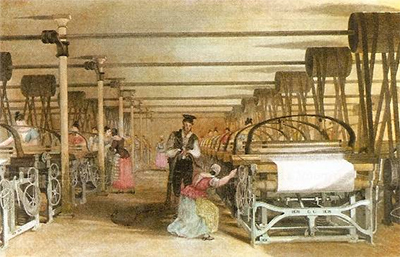
\includegraphics[width=0.9\linewidth]{Figuras/Ch01/fig1.jpg}}
}

\frame{
\frametitle{Histórico da automação}
\begin{block}{Revolução Industrial}
\begin{itemize}
    \item A tarefa do trabalhador era alimentar a máquina, controlar sua velocidade e zelar por sua manutenção. A principal consequência dessa organização foi a \textbf{dependência do homem em relação à tecnologia}. O trabalhador deixou de ser o dono dos instrumentos de trabalho e perdeu o conhecimento que tinha de todo o processo de produção.
\end{itemize}
\end{block}
}

\frame{
\frametitle{Histórico da automação}
\centerline{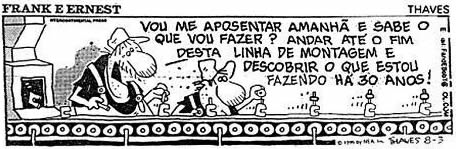
\includegraphics[width=1.1\linewidth]{Figuras/Ch01/fig2.jpg}}
}

\frame{
\frametitle{Histórico da automação}
\begin{block}{Linha de montagem}
\begin{itemize}
    \item Por volta de 1788, alguns tipos de artefatos mecânicos, sobretudo munidos de sistemas hidráulicos e pneumáticos passaram a ser aplicados nas \textbf{linhas de produção}, reduzindo esforços dos operadores, como também aumentando a precisão no controle do equipamento.
    \item Esses primeiros anos foram marcados por um impacto social muito grande, pois as máquinas realmente tomaram os postos de trabalhos e \textbf{só ficaram empregados aqueles que conseguiram se adaptar ou apresentaram maior aptidão para operar as máquinas}.
\end{itemize}
\end{block}
}

\frame{
\frametitle{Histórico da automação}
\begin{block}{Produção em série: Fordismo}
\begin{itemize}
    \item Já no século XX, houve o início da \textbf{produção em série}, sobretudo das técnicas desenvolvidas e aplicadas por \textbf{Henry Ford} nos Estados Unidos, de maneira que a indústria automobilística bateu recordes de produção de carros em menos tempo. Nesta época, o controle dos processos era realizado através de gigantescos e elaborados circuitos lógicos controlados por dispositivos eletromagnéticos \textbf{(relés)}.
\end{itemize}
\end{block}
}

\frame{
\frametitle{Histórico da automação}
\centerline{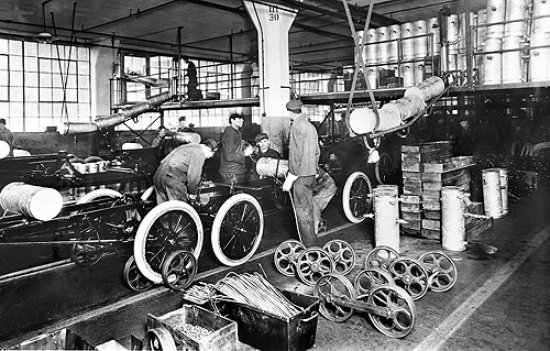
\includegraphics[width=0.9\linewidth]{Figuras/Ch01/fig3.jpg}}
}

\frame{
\frametitle{Histórico da automação}
\begin{block}{Produção em série: Fordismo}
\begin{itemize}
    \item Os sistemas controlados por lógicas de relés trouxeram um \textbf{grande avanço na automação} do processo produtivo dos automóveis. Entretanto haviam alguns \textbf{inconvenientes}:
    \begin{itemize}
        \item O \textbf{espaço} ocupado era imenso.
        \item Na ocorrência de um \textbf{defeito}, o diagnóstico era muito demorado. O pessoal da manutenção poderia levar dias para encontrar uma bobina queimada ou um contato defeituoso dentro do circuito.
        \item Quando era necessário \textbf{mudar o comportamento do sistema} (devido à mudança no modelo de carro produzido, por exemplo) era necessário sucatear todo o sistema e começar a fazer tudo do zero, o que custava meses de trabalho.
    \end{itemize}
\end{itemize}
\end{block}
}

\frame{
\frametitle{Histórico da automação}
\centerline{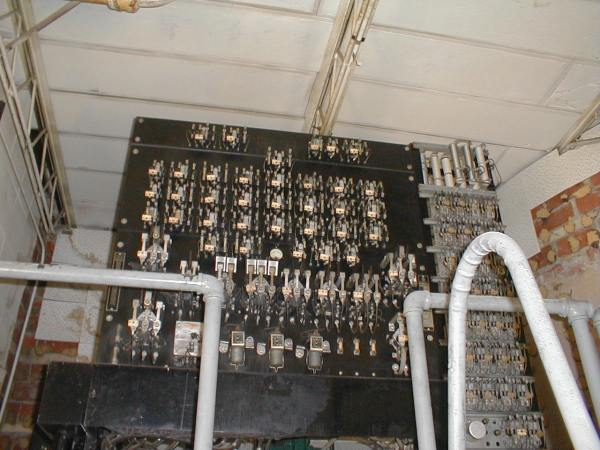
\includegraphics[width=0.7\linewidth]{Figuras/Ch01/fig4.jpg}}
}

\frame{
\frametitle{Histórico da automação}
\begin{block}{A eletrônica e os processadores}
\begin{itemize}
    \item Com o advento da \textbf{eletrônica} e com o aperfeiçoamento das técnicas e sistemas de medição e controle (instrumentação eletrônica) em meados da década de 50, as indústrias começaram a trabalhar com \textbf{equipamentos de controle ou comando numérico}, e o conceito de distribuição de \textbf{salas de controle} começou a ser difundido.
    \item Ressalta-se que em 1947, Willian Shockley, John Barden e Walter Brattain descobriram o \textbf{transistor}, que é um componente eletrônico utilizado aos bilhões nos processadores modernos.
    \item Com o aperfeiçoamento da eletrônica surgiram os primeiros \textbf{computadores industriais}, que começaram a ser utilizados na indústria a partir de 1961, quando também surgiram os primeiros \textbf{robôs industriais}.
\end{itemize}
\end{block}
}

\frame{
\frametitle{Histórico da automação}
\centerline{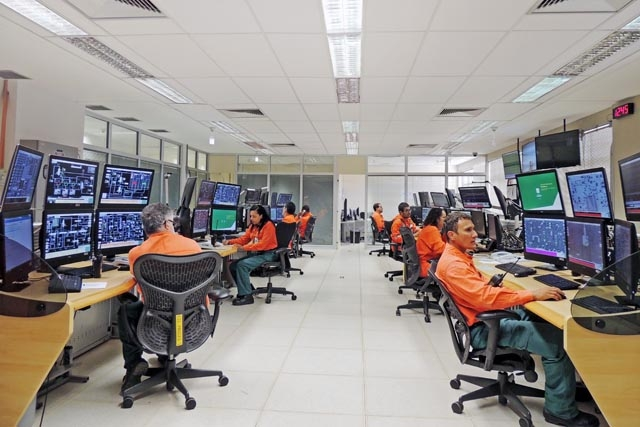
\includegraphics[width=0.9\linewidth]{Figuras/Ch01/fig5.jpg}}
}

\frame{
\frametitle{Histórico da automação}
\centerline{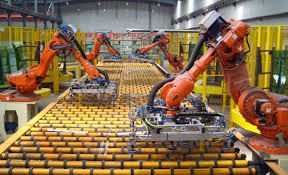
\includegraphics[width=0.9\linewidth]{Figuras/Ch01/fig6.jpg}}
}

\frame{
\frametitle{Histórico da automação}
\begin{block}{CLP}
\begin{itemize}
    \item O emprego de computadores na indústria de processos se justifica pelo fato de que o mesmo pode auxiliar no \textbf{aumento da produção e redução de gastos}, através da automação das máquinas. 
    \item Os microprocessadores podem tomar decisões de controle de uma máquina como ligá-la, desligá-la, movimentá-la, sinalizar defeitos e até gerar relatórios operacionais. Dentro deste conceito, surgiram \textbf{microcomputadores desenvolvidos especialmente} para efetuar operações e controles lógicos sobre os equipamentos com possibilidade de \textbf{reprogramação de suas funções}. Este microcomputador especial foi chamado de \textbf{PLC} (Programmable Logic Controller) ou em português, \textbf{CLP} (Controlador Lógico Programável).
\end{itemize}
\end{block}
}

\frame{
\frametitle{Histórico da automação}
\centerline{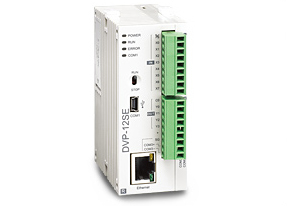
\includegraphics[width=0.9\linewidth]{Figuras/Ch01/fig7.jpg}}
}

\frame{
\frametitle{Definição}
\begin{block}{Afinal... o que é automação?}
\begin{itemize}
    \item \textbf{Etimologia}: \\
    Da palavra \textit{Automation} (1960), buscava enfatizar a participação do \textbf{computador} no controle automático industrial.
    \item \textbf{Definição atual}: \\
    “Qualquer sistema, apoiado em \textbf{computadores}, que substitui o trabalho humano, em favor da segurança das pessoas, da qualidade dos produtos, rapidez da produção ou da redução de custos, assim aperfeiçoando os complexos objetivos das indústrias, dos serviços ou bem estar” (Moraes e Castrucci, 2007).
\end{itemize}
\end{block}
}

\frame{
\frametitle{Aplicações}
\centerline{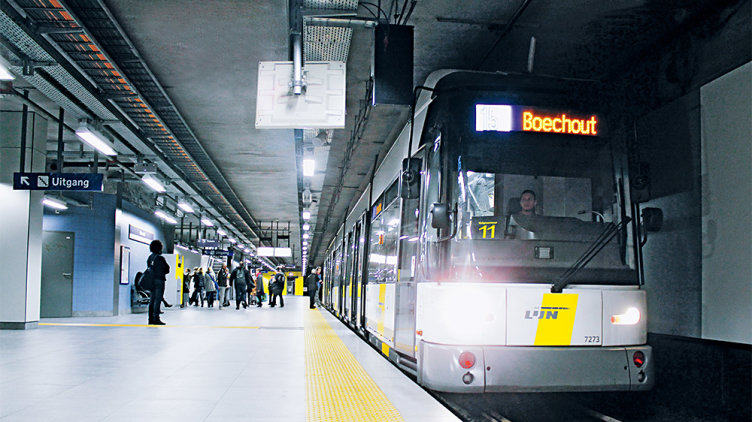
\includegraphics[width=0.9\linewidth]{Figuras/Ch01/fig8.jpg}}
\begin{block}{A automação em nossas vidas}
Quantos sistemas de automação você consegue identificar?
\end{block}
}

\frame{
\frametitle{Aplicações}
\centerline{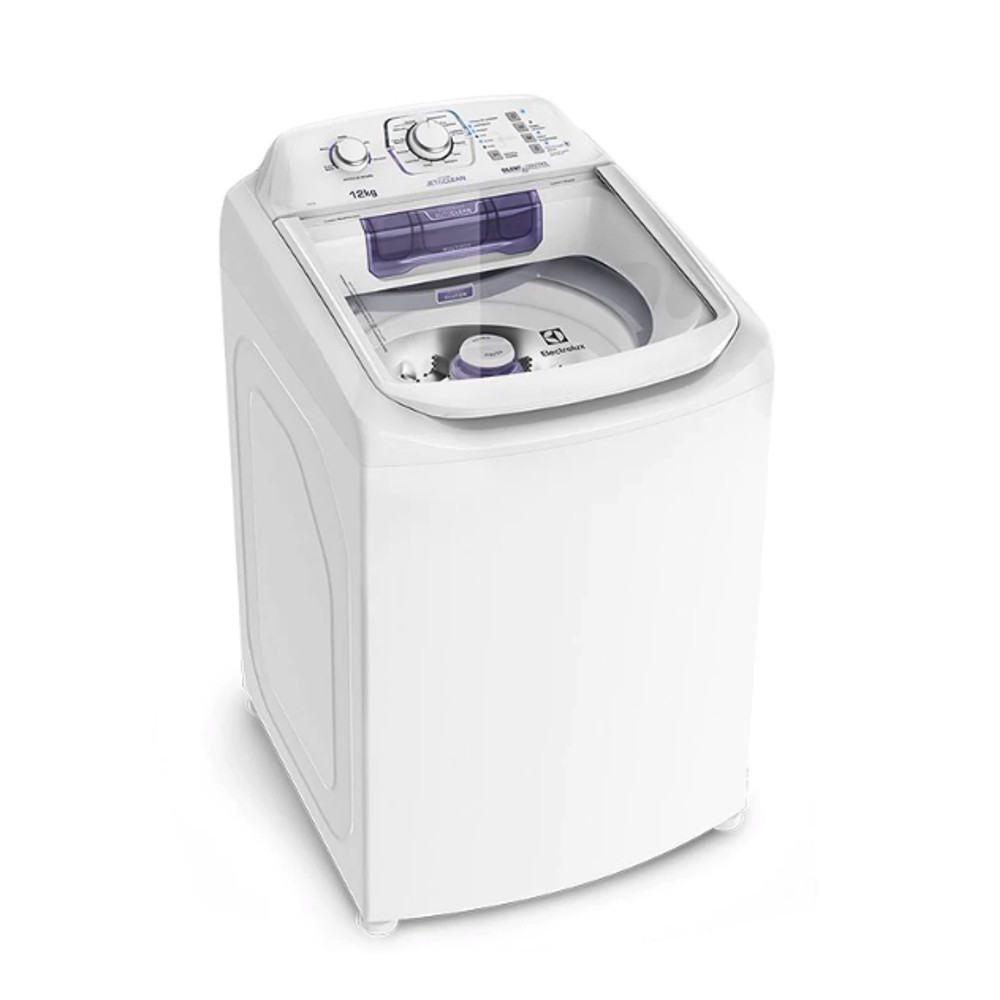
\includegraphics[width=0.6\linewidth]{Figuras/Ch01/fig9.jpg}}
}

\frame{
\frametitle{Aplicações}
\centerline{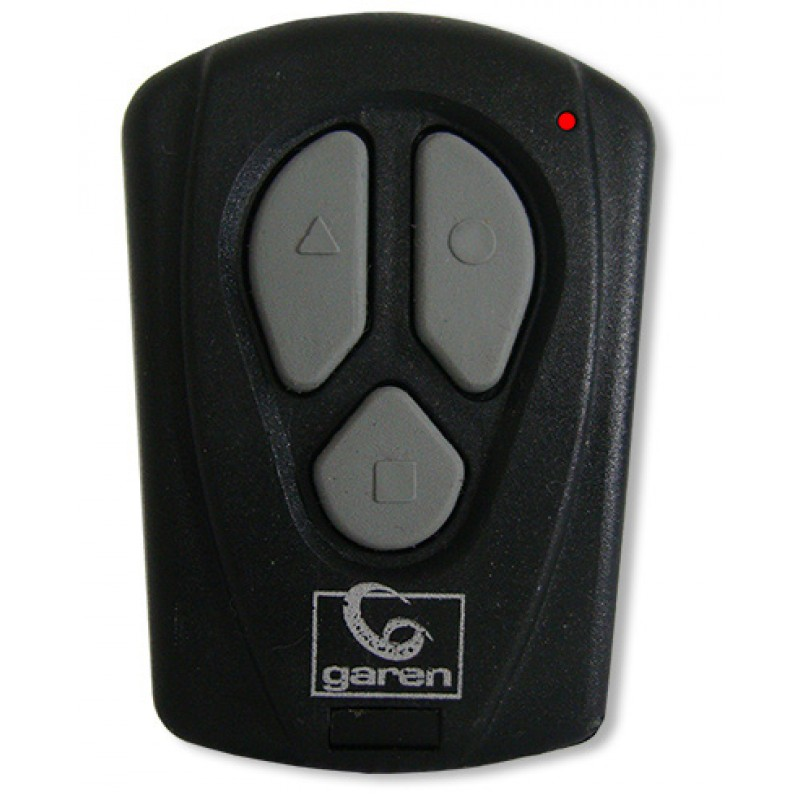
\includegraphics[width=0.4\linewidth]{Figuras/Ch01/fig10.jpg}}
}

\frame{
\frametitle{Aplicações}
\centerline{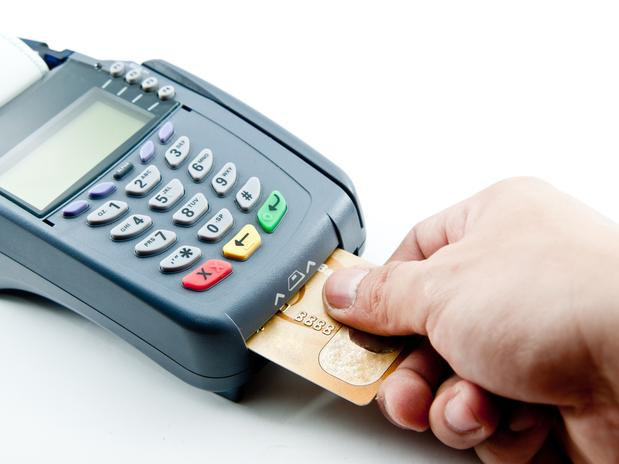
\includegraphics[width=0.7\linewidth]{Figuras/Ch01/fig11.jpg}}
}

\frame{
\frametitle{Aplicações}
\centerline{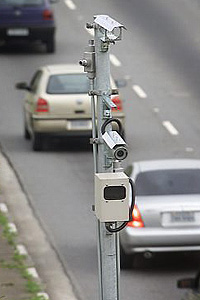
\includegraphics[width=0.4\linewidth]{Figuras/Ch01/fig12.jpg}}
}

\frame{
\frametitle{Aplicações}
\centerline{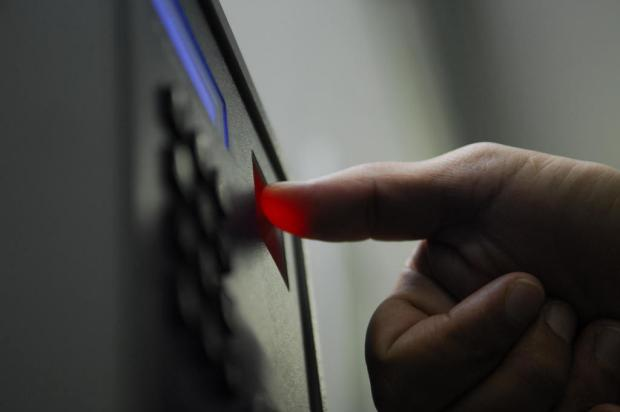
\includegraphics[width=0.9\linewidth]{Figuras/Ch01/fig13.jpg}}
}

\frame{
\frametitle{Aplicações}
\centerline{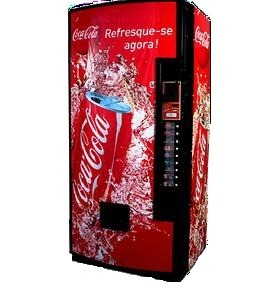
\includegraphics[width=0.6\linewidth]{Figuras/Ch01/fig14.jpg}}
}

\frame{
\frametitle{Características e conceitos da automação}
\begin{block}{Integração multidisciplinar}
Na Automação se reúnem três grandes áreas:
    \begin{enumerate}
        \item A \textbf{mecânica}, através das máquinas que possibilitam transformar matérias primas em produtos “acabados”.
        \item A \textbf{elétrica} que disponibiliza os motores, seus acionamentos e a eletrônica indispensável para o controle e automação das malhas de produção.
        \item A \textbf{informática} que através das arquiteturas de bancos de dados e redes de comunicação permitem disponibilizar as informações a todos os níveis de uma empresa.
    \end{enumerate}
\end{block}
}

\frame{
\frametitle{Características e conceitos da automação}
\centerline{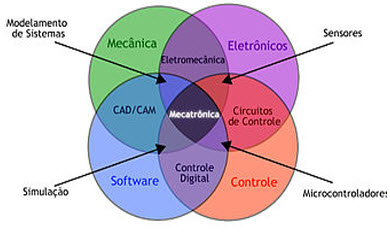
\includegraphics[width=0.9\linewidth]{Figuras/Ch01/fig15.jpg}}
}

\frame{
\frametitle{Características e conceitos da automação}
\begin{block}{Vantagens}
Assim, a automação, tão presente nas atividades humanas, está presente também nos
processos industriais, com o mesmo objetivo básico, que é \textbf{facilitar os processos produtivos}, permitindo produzir bens com:
    \begin{itemize}
        \item menor custo;
        \item maior quantidade;
        \item menor tempo;
        \item maior qualidade.
    \end{itemize}
\end{block}
}

\frame{
\frametitle{Características e conceitos da automação}
\begin{block}{Desempregos?}
    \begin{itemize}
        \item Novos tipos de trabalhos.
        \item “Uma máquina pode fazer uma determinada função, mas os trabalhos da maioria das pessoas envolvem várias funções diferentes. Você não pode automatizar todas as tarefas com uma única máquina.”
    \end{itemize}
\end{block}
}

\frame{
\frametitle{Áreas da automação}
\begin{block}{}
A automação é muito abrangente, e estuda desde portões eletrônicos até robótica na linha de produção. Para entendermos melhor, é preciso dividi-la em alguns \textbf{ramos principais}:
    \begin{itemize}
        \item \textbf{Automação Industrial}: procura escolher a tecnologia que melhor se adapta a uma máquina ou processo com a melhor relação de custo/benefício. Ela ainda pode ser subdividida em três níveis, sendo: de campo, de controle e de supervisão.
        \item \textbf{Automação Comercial}: nesse caso faz o uso de softwares para proporcionar a otimização de processos comerciais, desde a produção de sistemas de controle de estoque até a identificação de mercadorias por códigos de barra.
        \item \textbf{Automação Residencial}: aplicam-se as técnicas de automação para o conforto e a segurança habitacional, que variam desde o ajuste de temperatura por ar condicionado até o controle por biometria.
    \end{itemize}
\end{block}
}

\frame{
\frametitle{Áreas da automação}
\begin{block}{Domótica}
\textbf{Domótica} é uma tecnologia recente e é responsável pela gestão de todos os recursos habitacionais. Este termo nasceu da fusão da palavra \textit{domus}, que significa \textbf{casa}, com a palavra “Robótica”, que está ligada ao ato de automatizar, isto é, realizar ações de forma automática. 
\end{block}
\centerline{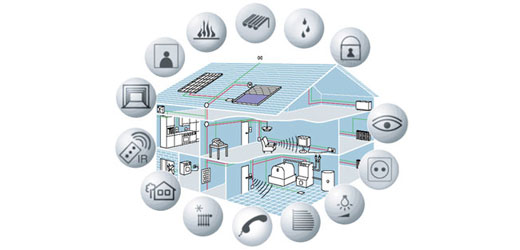
\includegraphics[width=0.9\linewidth]{Figuras/Ch01/fig16.jpg}}
}

\frame{
\frametitle{Áreas da automação}
\begin{block}{Aplicações da domótica}
\begin{itemize}
    \item Irrigação inteligente
    \item Controle de iluminação
    \item Cinema em casa
    \item Som ambiente
    \item Climatização
    \item Segurança
    \item Comunicação
\end{itemize}
\end{block}
}

\section*{Referências}
\frame{
\frametitle{Referências e Exercícios Complementares}
\begin{itemize}
\item FRANCHI, C. M. Controle de Processos Industriais: Princípios e Aplicações. 1 ed. São Paulo: Érica, 2011.
\end{itemize}
%\centering{\alert{Página 546 - \textbf{Capítulo 6}}} \\
%\centering{\alert{Lista de exercícios 01}}
}